\section{Diskussion}
\label{sec:Diskussion}

Aufgrund von Fehlen der tatsächlichen Abstände der Fehlstellen zu den Kanten und der Durchmesser
ist eine Auswertung der Genauigkeit der Scans nicht möglich. Auffällig ist jedoch, dass sich
die mittels A- und B-Scan ermittelten Durchmesser deutlich unterscheiden, was vielerlei
Ursache haben kann.
Allgemein können Fehler dadurch auftreten, dass die Schallgeschwindigkeit des
Materials der Schutzschicht nicht bekannt ist, dass das Koppelmittel (welches in der 
Berechnung ebenfalls vernachlässigt wurde) die Sonde nicht vollständig bedeckt hat, dass
die Literaturwerte der Schallgeschwindigkeit nicht exakt auf das benutzte Material zutreffen,
sowie menschliche Ungenauigkeit bei der Bestimmung der Laufzeiten durch manuelle Abmessung 
per Cursor.
Bei dem A-Scan war zudem nicht eindeutig zu erkennen, wo der Peak der reflektierten Schallwellen des Koppelmittels war.

\noindent Bei der Untersuchung des Auflösevermögens ist zu erkennen, dass mit steigender Frequenz die Auflösung zunimmt, da bei
der Messung mit 1MHz die Löcher 1 und 2 auf dem Diagramm nicht zu unterscheiden sind, was bei Nutzung von 2 oder 4
MHz der Fall ist. Allerdings ist auch zu erkennen, dass mit steigender Frequenz die Amplitude deutlich abnimmt, was
darauf hindeutet, dass diese genauere Messung nur für kürzere Laufzeiten realisierbar ist, sodass ein gewisser
Kompromiss eingegangen werden muss.

\noindent Bei der Messung des Herzvolumens konnte der Herzschlag gut simuliert werden, was sich in dem relativ konstanten Schlagvolumen
Schlagfrequenz widerspiegelt. Daher ergibt sich auch durch die Mittelung keine große Abweichung zu irgendeinem der gemessenen Werte. Soweit ist
die Berechnung des Herzvolumens also gut möglich. Es ist anzumerken, dass dennoch die Näherung durch ein Kugelsegment
als verdrängendem Volumen durchgeführt wurde, sodass der errechnete Wert trotz guter Bestimmbarkeit der Größe $h$ also
 nicht genau dem tatsächlichen Wert entsprechen wird. Verglichen mit dem Herzminutenvolumen eines
 erwachsenen Menschen, welches etwa $5\,\si{\liter\per\minute}$ beträgt\cite{kent4}, ergibt sich eine
 Abweichung von 99\%, was zum größten Teil an den deutlich kleineren Ausmaßen und dem damit kleineren verdrängten Volumen
 unseres Herzmodells und der verhältnismäßig niedrigen Schlagfrequenz liegt.

\begin{figure}[H]
  \centering
  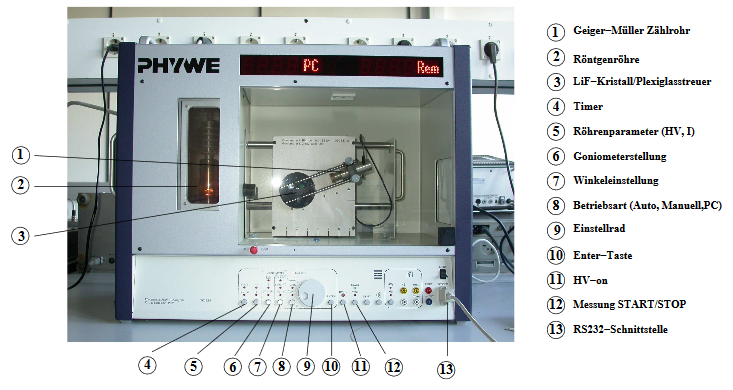
\includegraphics[height=5cm]{geraet.PNG}
  \caption{Das Röntgengerät. \cite[S.4]{kent}}
\end{figure}
 